% Options for packages loaded elsewhere
\PassOptionsToPackage{unicode}{hyperref}
\PassOptionsToPackage{hyphens}{url}
\PassOptionsToPackage{dvipsnames,svgnames,x11names}{xcolor}
%
\documentclass[
  letterpaper,
  DIV=11,
  numbers=noendperiod]{scrartcl}

\usepackage{amsmath,amssymb}
\usepackage{iftex}
\ifPDFTeX
  \usepackage[T1]{fontenc}
  \usepackage[utf8]{inputenc}
  \usepackage{textcomp} % provide euro and other symbols
\else % if luatex or xetex
  \usepackage{unicode-math}
  \defaultfontfeatures{Scale=MatchLowercase}
  \defaultfontfeatures[\rmfamily]{Ligatures=TeX,Scale=1}
\fi
\usepackage{lmodern}
\ifPDFTeX\else  
    % xetex/luatex font selection
\fi
% Use upquote if available, for straight quotes in verbatim environments
\IfFileExists{upquote.sty}{\usepackage{upquote}}{}
\IfFileExists{microtype.sty}{% use microtype if available
  \usepackage[]{microtype}
  \UseMicrotypeSet[protrusion]{basicmath} % disable protrusion for tt fonts
}{}
\makeatletter
\@ifundefined{KOMAClassName}{% if non-KOMA class
  \IfFileExists{parskip.sty}{%
    \usepackage{parskip}
  }{% else
    \setlength{\parindent}{0pt}
    \setlength{\parskip}{6pt plus 2pt minus 1pt}}
}{% if KOMA class
  \KOMAoptions{parskip=half}}
\makeatother
\usepackage{xcolor}
\setlength{\emergencystretch}{3em} % prevent overfull lines
\setcounter{secnumdepth}{-\maxdimen} % remove section numbering
% Make \paragraph and \subparagraph free-standing
\ifx\paragraph\undefined\else
  \let\oldparagraph\paragraph
  \renewcommand{\paragraph}[1]{\oldparagraph{#1}\mbox{}}
\fi
\ifx\subparagraph\undefined\else
  \let\oldsubparagraph\subparagraph
  \renewcommand{\subparagraph}[1]{\oldsubparagraph{#1}\mbox{}}
\fi

\usepackage{color}
\usepackage{fancyvrb}
\newcommand{\VerbBar}{|}
\newcommand{\VERB}{\Verb[commandchars=\\\{\}]}
\DefineVerbatimEnvironment{Highlighting}{Verbatim}{commandchars=\\\{\}}
% Add ',fontsize=\small' for more characters per line
\usepackage{framed}
\definecolor{shadecolor}{RGB}{241,243,245}
\newenvironment{Shaded}{\begin{snugshade}}{\end{snugshade}}
\newcommand{\AlertTok}[1]{\textcolor[rgb]{0.68,0.00,0.00}{#1}}
\newcommand{\AnnotationTok}[1]{\textcolor[rgb]{0.37,0.37,0.37}{#1}}
\newcommand{\AttributeTok}[1]{\textcolor[rgb]{0.40,0.45,0.13}{#1}}
\newcommand{\BaseNTok}[1]{\textcolor[rgb]{0.68,0.00,0.00}{#1}}
\newcommand{\BuiltInTok}[1]{\textcolor[rgb]{0.00,0.23,0.31}{#1}}
\newcommand{\CharTok}[1]{\textcolor[rgb]{0.13,0.47,0.30}{#1}}
\newcommand{\CommentTok}[1]{\textcolor[rgb]{0.37,0.37,0.37}{#1}}
\newcommand{\CommentVarTok}[1]{\textcolor[rgb]{0.37,0.37,0.37}{\textit{#1}}}
\newcommand{\ConstantTok}[1]{\textcolor[rgb]{0.56,0.35,0.01}{#1}}
\newcommand{\ControlFlowTok}[1]{\textcolor[rgb]{0.00,0.23,0.31}{#1}}
\newcommand{\DataTypeTok}[1]{\textcolor[rgb]{0.68,0.00,0.00}{#1}}
\newcommand{\DecValTok}[1]{\textcolor[rgb]{0.68,0.00,0.00}{#1}}
\newcommand{\DocumentationTok}[1]{\textcolor[rgb]{0.37,0.37,0.37}{\textit{#1}}}
\newcommand{\ErrorTok}[1]{\textcolor[rgb]{0.68,0.00,0.00}{#1}}
\newcommand{\ExtensionTok}[1]{\textcolor[rgb]{0.00,0.23,0.31}{#1}}
\newcommand{\FloatTok}[1]{\textcolor[rgb]{0.68,0.00,0.00}{#1}}
\newcommand{\FunctionTok}[1]{\textcolor[rgb]{0.28,0.35,0.67}{#1}}
\newcommand{\ImportTok}[1]{\textcolor[rgb]{0.00,0.46,0.62}{#1}}
\newcommand{\InformationTok}[1]{\textcolor[rgb]{0.37,0.37,0.37}{#1}}
\newcommand{\KeywordTok}[1]{\textcolor[rgb]{0.00,0.23,0.31}{#1}}
\newcommand{\NormalTok}[1]{\textcolor[rgb]{0.00,0.23,0.31}{#1}}
\newcommand{\OperatorTok}[1]{\textcolor[rgb]{0.37,0.37,0.37}{#1}}
\newcommand{\OtherTok}[1]{\textcolor[rgb]{0.00,0.23,0.31}{#1}}
\newcommand{\PreprocessorTok}[1]{\textcolor[rgb]{0.68,0.00,0.00}{#1}}
\newcommand{\RegionMarkerTok}[1]{\textcolor[rgb]{0.00,0.23,0.31}{#1}}
\newcommand{\SpecialCharTok}[1]{\textcolor[rgb]{0.37,0.37,0.37}{#1}}
\newcommand{\SpecialStringTok}[1]{\textcolor[rgb]{0.13,0.47,0.30}{#1}}
\newcommand{\StringTok}[1]{\textcolor[rgb]{0.13,0.47,0.30}{#1}}
\newcommand{\VariableTok}[1]{\textcolor[rgb]{0.07,0.07,0.07}{#1}}
\newcommand{\VerbatimStringTok}[1]{\textcolor[rgb]{0.13,0.47,0.30}{#1}}
\newcommand{\WarningTok}[1]{\textcolor[rgb]{0.37,0.37,0.37}{\textit{#1}}}

\providecommand{\tightlist}{%
  \setlength{\itemsep}{0pt}\setlength{\parskip}{0pt}}\usepackage{longtable,booktabs,array}
\usepackage{calc} % for calculating minipage widths
% Correct order of tables after \paragraph or \subparagraph
\usepackage{etoolbox}
\makeatletter
\patchcmd\longtable{\par}{\if@noskipsec\mbox{}\fi\par}{}{}
\makeatother
% Allow footnotes in longtable head/foot
\IfFileExists{footnotehyper.sty}{\usepackage{footnotehyper}}{\usepackage{footnote}}
\makesavenoteenv{longtable}
\usepackage{graphicx}
\makeatletter
\def\maxwidth{\ifdim\Gin@nat@width>\linewidth\linewidth\else\Gin@nat@width\fi}
\def\maxheight{\ifdim\Gin@nat@height>\textheight\textheight\else\Gin@nat@height\fi}
\makeatother
% Scale images if necessary, so that they will not overflow the page
% margins by default, and it is still possible to overwrite the defaults
% using explicit options in \includegraphics[width, height, ...]{}
\setkeys{Gin}{width=\maxwidth,height=\maxheight,keepaspectratio}
% Set default figure placement to htbp
\makeatletter
\def\fps@figure{htbp}
\makeatother

\KOMAoption{captions}{tableheading}
\makeatletter
\@ifpackageloaded{caption}{}{\usepackage{caption}}
\AtBeginDocument{%
\ifdefined\contentsname
  \renewcommand*\contentsname{Table of contents}
\else
  \newcommand\contentsname{Table of contents}
\fi
\ifdefined\listfigurename
  \renewcommand*\listfigurename{List of Figures}
\else
  \newcommand\listfigurename{List of Figures}
\fi
\ifdefined\listtablename
  \renewcommand*\listtablename{List of Tables}
\else
  \newcommand\listtablename{List of Tables}
\fi
\ifdefined\figurename
  \renewcommand*\figurename{Figure}
\else
  \newcommand\figurename{Figure}
\fi
\ifdefined\tablename
  \renewcommand*\tablename{Table}
\else
  \newcommand\tablename{Table}
\fi
}
\@ifpackageloaded{float}{}{\usepackage{float}}
\floatstyle{ruled}
\@ifundefined{c@chapter}{\newfloat{codelisting}{h}{lop}}{\newfloat{codelisting}{h}{lop}[chapter]}
\floatname{codelisting}{Listing}
\newcommand*\listoflistings{\listof{codelisting}{List of Listings}}
\makeatother
\makeatletter
\makeatother
\makeatletter
\@ifpackageloaded{caption}{}{\usepackage{caption}}
\@ifpackageloaded{subcaption}{}{\usepackage{subcaption}}
\makeatother
\ifLuaTeX
  \usepackage{selnolig}  % disable illegal ligatures
\fi
\usepackage{bookmark}

\IfFileExists{xurl.sty}{\usepackage{xurl}}{} % add URL line breaks if available
\urlstyle{same} % disable monospaced font for URLs
\hypersetup{
  pdftitle={STA310 HW3},
  pdfauthor={Olivia Fu},
  colorlinks=true,
  linkcolor={blue},
  filecolor={Maroon},
  citecolor={Blue},
  urlcolor={Blue},
  pdfcreator={LaTeX via pandoc}}

\title{STA310 HW3}
\author{Olivia Fu}
\date{2025-02-07}

\begin{document}
\maketitle

\begin{Shaded}
\begin{Highlighting}[]
\FunctionTok{library}\NormalTok{(ggplot2)}
\end{Highlighting}
\end{Shaded}

\subsection{Exercise 1}\label{exercise-1}

The probability mass function of a Poisson random variable is given by:

\[
P(X = x) = \frac{\lambda^x e^{-\lambda}}{x!}, \quad x = 0, 1, 2, \dots
\]

The likelihood function is:

\[
\begin{aligned}L(\lambda) &= \prod_{i=1}^n P(X_i = x_i)\\&= \prod_{i=1}^n \frac{\lambda^{x_i} e^{-\lambda}}{x_i!}\\&= \lambda^{\sum_{i=1}^n x_i} \cdot e^{-n\lambda} \cdot \prod_{i=1}^n \frac{1}{x_i!}\end{aligned}
\]

\clearpage

\subsection{Exercise 2}\label{exercise-2}

The log-likelihood function is:

\[
\begin{aligned}\ell(\lambda) &= \log L(\lambda) \\&=\log \left( \lambda^{\sum_{i=1}^n x_i}\cdot e^{-n\lambda} \cdot \prod_{i=1}^n \frac{1}{x_i!} \right)\\&= \log(\lambda^{\sum_{i=1}^n x_i}) + \log(e^{-n\lambda}) + \log(\prod_{i=1}^n \frac{1}{x_i!})\\&= \sum_{i=1}^n x_i \cdot \log \lambda - n\lambda + \sum_{i=1}^n \log \frac{1}{x_i!}\end{aligned}
\]

The first derivative of the log-likelihood function is:

\[
\frac{\partial \ell(\lambda)}{\partial \lambda} = \frac{\sum_{i=1}^n x_i}{\lambda} - n
\]

We then set the derivative equal to zero to find the MLE:

\[
\begin{aligned} \frac{\sum_{i=1}^n x_i}{\hat{\lambda}} - n = 0& \\\hat{\lambda} = \frac{\sum_{i=1}^n x_i}{n}&\end{aligned}
\]

The second derivative of the log-likelihood function is:

\[
\frac{\partial^2 \ell(\lambda)}{\partial \lambda^2} = -\frac{\sum_{i=1}^n x_i}{\lambda^2}
\]

Since \(\lambda > 0\) and \(x_i \geq 0\), the second derivative is
negative (exclude the trivial case where all \(x_i=0\)), confirming that
the critical point corresponds to a maximum.

\clearpage

\subsection{Exercise 3}\label{exercise-3}

\begin{Shaded}
\begin{Highlighting}[]
\CommentTok{\# Given data}
\NormalTok{n }\OtherTok{\textless{}{-}} \DecValTok{100}
\NormalTok{sum\_x }\OtherTok{\textless{}{-}} \DecValTok{500}

\CommentTok{\# Log{-}likelihood function for Poisson distribution}
\NormalTok{log\_likelihood\_function }\OtherTok{\textless{}{-}} \ControlFlowTok{function}\NormalTok{(lambda) \{}
  \ControlFlowTok{if}\NormalTok{ (lambda }\SpecialCharTok{\textless{}=} \DecValTok{0}\NormalTok{) \{}
    \FunctionTok{return}\NormalTok{(}\SpecialCharTok{{-}}\ConstantTok{Inf}\NormalTok{)}
\NormalTok{  \} }\ControlFlowTok{else}\NormalTok{ \{}
    \CommentTok{\# The constant term can be ignored as }
    \CommentTok{\# it does not affect the maximization of the log{-}likelihood}
    \FunctionTok{return}\NormalTok{(sum\_x }\SpecialCharTok{*} \FunctionTok{log}\NormalTok{(lambda) }\SpecialCharTok{{-}}\NormalTok{ n }\SpecialCharTok{*}\NormalTok{ lambda)}
\NormalTok{  \}}
\NormalTok{\}}

\CommentTok{\# Set up a sequence of lambda values}
\NormalTok{lambda\_values }\OtherTok{\textless{}{-}} \FunctionTok{seq}\NormalTok{(}\DecValTok{1}\NormalTok{, }\DecValTok{10}\NormalTok{, }\AttributeTok{length.out =} \DecValTok{100000}\NormalTok{)}

\CommentTok{\# Calculate the log{-}likelihood for each lambda}
\NormalTok{log\_likelihood\_values }\OtherTok{\textless{}{-}} \FunctionTok{sapply}\NormalTok{(lambda\_values, log\_likelihood\_function)}

\CommentTok{\# Find the lambda that maximizes the log{-}likelihood}
\NormalTok{mle\_lambda }\OtherTok{\textless{}{-}}\NormalTok{ lambda\_values[}\FunctionTok{which.max}\NormalTok{(log\_likelihood\_values)]}

\CommentTok{\# Print the MLE for lambda}
\FunctionTok{cat}\NormalTok{(}\StringTok{"MLE for lambda:"}\NormalTok{, mle\_lambda, }\StringTok{"}\SpecialCharTok{\textbackslash{}n}\StringTok{"}\NormalTok{)}
\end{Highlighting}
\end{Shaded}

\begin{verbatim}
MLE for lambda: 5 
\end{verbatim}

\begin{Shaded}
\begin{Highlighting}[]
\CommentTok{\# Create a dataframe}
\NormalTok{data }\OtherTok{\textless{}{-}} \FunctionTok{data.frame}\NormalTok{(}\AttributeTok{lambda =}\NormalTok{ lambda\_values, }\AttributeTok{log\_likelihood =}\NormalTok{ log\_likelihood\_values)}

\CommentTok{\# Plot}
\FunctionTok{ggplot}\NormalTok{(data, }\FunctionTok{aes}\NormalTok{(}\AttributeTok{x =}\NormalTok{ lambda, }\AttributeTok{y =}\NormalTok{ log\_likelihood)) }\SpecialCharTok{+}
  \FunctionTok{geom\_line}\NormalTok{(}\AttributeTok{color =} \StringTok{"blue"}\NormalTok{, }\AttributeTok{size =} \DecValTok{1}\NormalTok{) }\SpecialCharTok{+}
  \FunctionTok{geom\_vline}\NormalTok{(}\AttributeTok{xintercept =}\NormalTok{ mle\_lambda, }\AttributeTok{color =} \StringTok{"red"}\NormalTok{, }\AttributeTok{linetype =} \StringTok{"dashed"}\NormalTok{) }\SpecialCharTok{+}
  \FunctionTok{annotate}\NormalTok{(}\StringTok{"text"}\NormalTok{, }
           \AttributeTok{x =}\NormalTok{ mle\_lambda }\SpecialCharTok{+} \FloatTok{0.6}\NormalTok{, }
           \AttributeTok{y =} \FunctionTok{max}\NormalTok{(log\_likelihood\_values) }\SpecialCharTok{{-}} \DecValTok{40}\NormalTok{,}
           \AttributeTok{label =} \FunctionTok{paste}\NormalTok{(}\StringTok{"MLE ="}\NormalTok{, }\FunctionTok{round}\NormalTok{(mle\_lambda, }\DecValTok{3}\NormalTok{)), }
           \AttributeTok{color =} \StringTok{"red"}\NormalTok{) }\SpecialCharTok{+}
  \FunctionTok{labs}\NormalTok{(}\AttributeTok{title =} \StringTok{"Log{-}Likelihood for Poisson"}\NormalTok{,}
       \AttributeTok{x =} \StringTok{"Lambda"}\NormalTok{,}
       \AttributeTok{y =} \StringTok{"Log{-}Likelihood"}\NormalTok{) }\SpecialCharTok{+}
  \FunctionTok{theme\_minimal}\NormalTok{()}
\end{Highlighting}
\end{Shaded}

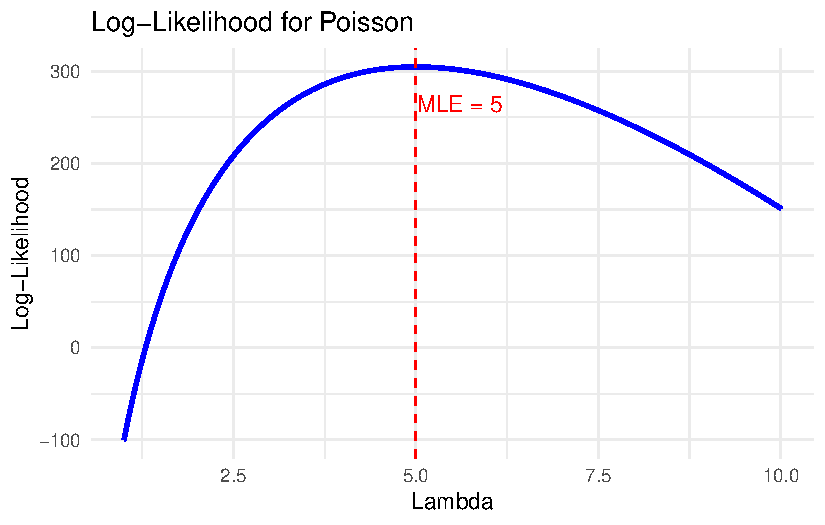
\includegraphics{HW3_files/figure-pdf/unnamed-chunk-4-1.pdf}

Therefore, the approximate MLE is 5, which matches the formula we
derived in Exercise 2.

\[
\hat{\lambda} = \frac{\sum_{i=1}^n x_i}{n} = \frac{500}{100}=5
\]

\clearpage

\subsection{Exercise 4}\label{exercise-4}

\subsubsection{(a)}\label{a}

\begin{longtable}[]{@{}
  >{\raggedright\arraybackslash}p{(\columnwidth - 6\tabcolsep) * \real{0.2083}}
  >{\raggedright\arraybackslash}p{(\columnwidth - 6\tabcolsep) * \real{0.2083}}
  >{\raggedright\arraybackslash}p{(\columnwidth - 6\tabcolsep) * \real{0.2083}}
  >{\raggedright\arraybackslash}p{(\columnwidth - 6\tabcolsep) * \real{0.3750}}@{}}
\toprule\noalign{}
\begin{minipage}[b]{\linewidth}\raggedright
\textbf{Game}
\end{minipage} & \begin{minipage}[b]{\linewidth}\raggedright
\textbf{First five shots}
\end{minipage} & \begin{minipage}[b]{\linewidth}\raggedright
\textbf{Likelihood (no hot hand)}
\end{minipage} & \begin{minipage}[b]{\linewidth}\raggedright
\textbf{Likelihood (hot hand)}
\end{minipage} \\
\midrule\noalign{}
\endhead
\bottomrule\noalign{}
\endlastfoot
1 & BMMBB & \(p_B^3(1 - p_B)^2\) &
\((p_B)(1-p_{B\vert B})(1-p_B)(p_B)(p_{B\vert B}) = (p_B)^2(1-p_{B\vert B})(1-p_B)(p_{B\vert B})\) \\
2 & MBMBM & \(p_B^2(1 - p_B)^3\) &
\((1-p_B)(p_B)(1-p_{B\vert B})(p_B)(1-p_{B\vert B}) = (p_B)^2(1-p_{B\vert B})^2(1-p_B)\) \\
3 & MMBBB & \(p_B^3(1 - p_B)^2\) &
\((1-p_B)(1-p_B)(p_B)(p_{B\vert B})(p_{B\vert B}) = (p_B)(1-p_B)^2(p_{B\vert B})^2\) \\
4 & BMMMB & \(p_B^2(1 - p_B)^3\) &
\((p_B)(1-p_{B\vert B})(1-p_B)(1-p_B)(p_B) = (p_B)^2(1-p_{B\vert B})(1-p_B)^2\) \\
5 & MMMMM & \((1 - p_B)^5\) &
\((1-p_B)(1-p_B)(1-p_B)(1-p_B)(1-p_B) = (1-p_B)^5\) \\
& & & \\
\textbf{Total} & & \(p_B^{10}(1 - p_B)^{15}\) &
\((p_B)^7(1-p_B)^{11}(p_{B\vert B})^3(1-p_{B\vert B})^4\) \\
\end{longtable}

\subsubsection{(b)}\label{b}

\begin{Shaded}
\begin{Highlighting}[]
\NormalTok{likelihood }\OtherTok{\textless{}{-}} \ControlFlowTok{function}\NormalTok{(pb)\{}
\NormalTok{  pb}\SpecialCharTok{\^{}}\NormalTok{(}\DecValTok{10}\NormalTok{) }\SpecialCharTok{*}\NormalTok{ (}\DecValTok{1} \SpecialCharTok{{-}}\NormalTok{ pb)}\SpecialCharTok{\^{}}\NormalTok{(}\DecValTok{15}\NormalTok{)}
\NormalTok{\}}
\FunctionTok{likelihood}\NormalTok{(}\FloatTok{0.4}\NormalTok{)}
\end{Highlighting}
\end{Shaded}

\begin{verbatim}
[1] 4.930247e-08
\end{verbatim}

\begin{Shaded}
\begin{Highlighting}[]
\FunctionTok{likelihood}\NormalTok{(}\FloatTok{0.3}\NormalTok{)}
\end{Highlighting}
\end{Shaded}

\begin{verbatim}
[1] 2.803388e-08
\end{verbatim}

When we substitute 0.4 and 0.3 for \(p_B\)\hspace{0pt} in the likelihood
function, we find that \(p_B=0.4\) produces a higher likelihood than
\(p_B=0.3\) (\(4.93 \times 10^{-8}\) vs.~\(2.80 \times 10^{-8}\)). This
means that the data is more consistent with \(p_B=0.4\).

Furthermore, intuitively, if the data shows that the player made 10
baskets out of 25 attempts, it makes sense to estimate the probability
of making a basket close to 0.4 (10/25), rather than lower values like
0.3, which are less aligned with the observed data.

\subsubsection{(c)}\label{c}

\textbf{MLE for No Hot Hand Model}

The likelihood and log-likelihood functions are:

\[
\begin{aligned}Lik(p_B) &= p_B^{10}(1 - p_B)^{15}\\\log(Lik(p_B)) &= \log(p_B^{10})+\log((1 - p_B)^{15})\\&= 10\log(p_B) + 15\log(1 - p_B)\end{aligned}
\]

We then take the first derivative of the log-likelihood function and set
it to zero:

\[
\begin{aligned}\frac{d}{dp_B}log(Lik(p_B)) &= \frac{10}{p_B}-\frac{15}{1-p_B} = 0\\&\Rightarrow \frac{10}{p_B} = \frac{15}{1-p_B}\\&\Rightarrow 10(1-p_B)=15p_B\\&\Rightarrow 25p_B = 10\\&\hat{p_B} = \frac{10}{25} = 0.4\end{aligned}
\]

\textbf{MLE for Hot Hand Model}

The likelihood and log-likelihood functions are:

\[
$\begin{aligned}Lik(p_B, p_{B\vert B}) &= (p_B)^7(1-p_B)^{11}(p_{B\vert B})^3(1-p_{B\vert B})^4\\\log(Lik(p_B, p_{B\vert B})) &= \log((p_B)^7)+\log((1-p_B)^{11})+\log((p_{B\vert B})^3)+\log((1-p_{B\vert B})^4)\\&= 7\log((p_B))+11\log((1-p_B))+3\log((p_{B\vert B}))+4\log((1-p_{B\vert B}))\end{aligned}$
\]

We then take the first derivative of the log-likelihood function (with
respect to \(p_B\) and \(p_{B \vert B}\) separately) and set them to
zero:

\[
\begin{aligned}\frac{d}{dp_B}log(Lik(p_B, p_{B\vert B})) &= \frac{7}{p_B}-\frac{11}{1-p_B} = 0\\&\Rightarrow \frac{7}{p_B} = \frac{11}{1-p_B}\\&\Rightarrow 7(1-p_B)=11p_B\\&\Rightarrow 18p_B = 7\\&\hat{p_B} = \frac{7}{18} = 0.3889\\\\\frac{d}{dp_{B\vert B}}log(Lik(p_B, p_{B\vert B})) &= \frac{3}{p_{B\vert B}}-\frac{4}{1-p_{B\vert B}} = 0\\&\Rightarrow \frac{3}{p_{B\vert B}} = \frac{4}{1-p_{B\vert B}}\\&\Rightarrow 3(1-p_{B\vert B})=4p_{B\vert B}\\&\Rightarrow 7p_{B\vert B} = 3\\&\hat{p_{B \vert B}} = \frac{3}{7} = 0.4286\end{aligned}
\]

\textbf{Likelihood Ratio Test (LRT)}

No Hot Hand Model: \(p_B\)

Hot Hand Model: \(p_B, p_{B \vert B}\)

Hypothesis:

\(H_0:p_B=p_{B \vert B}\)

\(H_0:p_B \neq p_{B \vert B}\)

Firstly, we need to plug the MLEs into the log-likelihood function for
each model to get the maximum value of the log-likelihood for each
model.

\begin{Shaded}
\begin{Highlighting}[]
\NormalTok{loglik1 }\OtherTok{\textless{}{-}} \ControlFlowTok{function}\NormalTok{(pb)\{}
  \FunctionTok{log}\NormalTok{(pb}\SpecialCharTok{\^{}}\NormalTok{(}\DecValTok{10}\NormalTok{) }\SpecialCharTok{*}\NormalTok{ (}\DecValTok{1} \SpecialCharTok{{-}}\NormalTok{ pb)}\SpecialCharTok{\^{}}\NormalTok{(}\DecValTok{15}\NormalTok{))}
\NormalTok{\}}
\FunctionTok{loglik1}\NormalTok{(}\DecValTok{10}\SpecialCharTok{/}\DecValTok{25}\NormalTok{)}
\end{Highlighting}
\end{Shaded}

\begin{verbatim}
[1] -16.82529
\end{verbatim}

\begin{Shaded}
\begin{Highlighting}[]
\NormalTok{loglik2 }\OtherTok{\textless{}{-}} \ControlFlowTok{function}\NormalTok{(pb, pbb) \{}
  \FunctionTok{log}\NormalTok{(pb}\SpecialCharTok{\^{}}\DecValTok{7} \SpecialCharTok{*}\NormalTok{ (}\DecValTok{1}\SpecialCharTok{{-}}\NormalTok{pb)}\SpecialCharTok{\^{}}\NormalTok{(}\DecValTok{11}\NormalTok{) }\SpecialCharTok{*}\NormalTok{ pbb}\SpecialCharTok{\^{}}\DecValTok{3} \SpecialCharTok{*}\NormalTok{ (}\DecValTok{1}\SpecialCharTok{{-}}\NormalTok{pbb)}\SpecialCharTok{\^{}}\DecValTok{4}\NormalTok{)}
\NormalTok{\}}
\FunctionTok{loglik2}\NormalTok{(}\DecValTok{7}\SpecialCharTok{/}\DecValTok{18}\NormalTok{, }\DecValTok{3}\SpecialCharTok{/}\DecValTok{7}\NormalTok{)}
\end{Highlighting}
\end{Shaded}

\begin{verbatim}
[1] -16.80883
\end{verbatim}

Then, we use the Likelihood Ratio Test to determine if the difference is
statistically significant

\begin{Shaded}
\begin{Highlighting}[]
\NormalTok{LRT }\OtherTok{\textless{}{-}} \DecValTok{2} \SpecialCharTok{*}\NormalTok{ (}\FunctionTok{loglik2}\NormalTok{(}\DecValTok{7}\SpecialCharTok{/}\DecValTok{18}\NormalTok{, }\DecValTok{3}\SpecialCharTok{/}\DecValTok{7}\NormalTok{) }\SpecialCharTok{{-}} \FunctionTok{loglik1}\NormalTok{(}\DecValTok{10}\SpecialCharTok{/}\DecValTok{25}\NormalTok{))}
\NormalTok{LRT}
\end{Highlighting}
\end{Shaded}

\begin{verbatim}
[1] 0.03292469
\end{verbatim}

Therefore, LRT = 0.03292.

The test statistic follows a \(\chi^2\) distribution with 1 degrees of
freedom (the difference in the number of parameters between the two
models). Therefore, the p-value is \(P(\chi^2>LRT)\).

\begin{Shaded}
\begin{Highlighting}[]
\FunctionTok{pchisq}\NormalTok{(LRT, }\DecValTok{1}\NormalTok{, }\AttributeTok{lower.tail =} \ConstantTok{FALSE}\NormalTok{)}
\end{Highlighting}
\end{Shaded}

\begin{verbatim}
[1] 0.8560131
\end{verbatim}

Therefore, p-value = 0.8560.

The p-value is very larger, so we fail to reject \(H_0\). We don't have
convincing evidence that the hot hand model (conditional model) is an
improvement over the no hot hand model (unconditional model). Thus,
\textbf{there is no significant evidence that the hod hand exists}.



\end{document}
